In this section we present some preliminary results and point out certain patterns
that appear in our data. 

\subsection*{Overheads} Whether an expression is worthwhile to evaluate in
parallel is directly tied to \emph{cost} of creating a parallel task. Because
our search algorithm is not deterministic, we do not have the statistical
issues that were present in the previous chapter. Therefore we took the
opportunity to experiment with various overheads as well.

Based on the benchmarking of GHC's \verb|par| we have chosen a lower and upper
bound.  While the lower bound ($10$) and the upper bound ($1000$) are both
unrealistic (i.e. benchmarking GHC points to the actual overhead being
somewhere in the hundreds of reductions) this will help us see how sensitive
our approach is to the overhead of a \verb|par|.


\subsection*{Experimental Results}

For each program we set our runtime system to simulate 4, 8, and 16 cores.
First, let us examine Figure \ref{table10} which displays the results of setting
the cost of task creation to 10 reductions.

\begin{table}[ht]
\caption[Profile-Directed Search with an overhead of $10$ reductions]{Speedups relative to sequential computation when the cost of sparking
        a task is set to 10 reductions. The number of runs corresponds to the
        number of \texttt{par} sites that have been switched off.}
\centering
\smallskip
  \begin{tabular}{ l||c c c c c c  }
    Program & \multicolumn{2}{c}{4-core} & \multicolumn{2}{c}{8-cores} & \multicolumn{2}{c}{16-cores} \\
            & Runs & Final     & Runs & Final      & Runs & Final \\
    \hline
    SumEuler  & 6    & 3.77      & 6    & 6.84       & 6    & 10.27     \\
    Queens    & 5    & 1.30      & 5    & 1.37       & 5    & 1.41  \\
    Queens2   & 22   & 3.91      & 22   & 7.74       & 22   & 15.07   \\
    SodaCount & 3    & 2.42      & 3    & 4.72       & 3    & 8.95    \\
    Tak       & 1    & 3.39      & 1    & 6.79       & 1    & 13.58   \\
    Taut      & 4    & 1.00      & 0    & 1.00       & 9    & 1.00  \\
    MatMul    & 2    & 1.02      & 2    & 1.07       & 2    & 1.10   \\
  \end{tabular}
\label{table10}
\end{table}

Already there are a few interesting results. \verb|SumEuler| performs as
expected and manages to eliminate the majority of the introduced \verb-par-
sites. Interestingly, the \verb|par| sites that remain are, when taken
together, equivalent to applying \verb-parMap euler- over the input
list\footnote{See Appendix \ref{append:bench} for the source of the program.}.
When this program is parallelised explicitly, that \verb-parMap- is usually the
only addition to the program \citep{vGMachine}. It is reassuring that our
technique converges on the same result.

The two implementations of \verb|nQueens| vary drastically in their
improvement, with the more symbolic solution (\verb|Queens2|) achieving much
better results. Search problems are known to be problematic for techniques
involving strictness analysis and usually benefit from the introduction of
\emph{speculative} parallelism \citep{hammond2000research}.

\verb|Taut| was chosen as a benchmark program specifically because the program (as
written) did not have many opportunities for parallelism. Had our technique
managed to find any useful parallelism, we would have been surprised.

\verb|MatMul| is, to us, the most surprising of the results so far. Matrix
multiplication is famously parallelisable and yet our implementation barely
breaks even! Notice that of the 7 \verb-par- sites in \verb|MatMul|, only 2 are
being switched off. We will investigate \verb|MatMul|'s performance in a bit
more depth in Section \ref{sec:limits}.

While the results in Figure \ref{table10} are revealing, it could be argued that
an overhead of 10 reductions to spark off a thread is unrealistically low.
Therefore we repeat the experiments with the more realistic 100 reduction
overhead (Figure \ref{table100}) and the pessimistic case of 1000 reduction
overheads (Figure \ref{table1000}).

\begin{table}[ht]
\caption[Profile-Directed Search with overheads of $100$ reductions]{Speedups relative to sequential computation when the cost of sparking
        a task is set to 100 reductions. The number of runs corresponds to the
        number of \texttt{par} sites that have been switched off.}
\centering
\smallskip
  \begin{tabular}{ l||c c c c c c  }
    Program & \multicolumn{2}{c}{4-core} & \multicolumn{2}{c}{8-cores} & \multicolumn{2}{c}{16-cores} \\
            & Runs & Final     & Runs & Final      & Runs & Final \\
    \hline
    SumEuler  & 6    & 3.74      & 6    & 6.81       & 6    & 10.23     \\
    Queens    & 5    & 1.29      & 5    & 1.37       & 5    & 1.41  \\
    Queens2   & 22   & 3.83      & 22   & 7.57       & 22   & 14.76  \\
    SodaCount & 3    & 2.17      & 3    & 4.23       & 3    & 8.02    \\
    Tak       & 1    & 2.36      & 1    & 4.71       & 1    & 9.42   \\
    Taut      & 9    & 1.00      & 0    & 1.00       & 9    & 1.00  \\
    MatMul    & 2    & 0.93      & 2    & 1.06       & 2    & 1.09   \\
  \end{tabular}
\label{table100}
\end{table}

The results in Figure \ref{table100} mostly align with what we would expect to
happen if creating a parallel task incurred higher overheads: we see reduced
speedup factors and adding more cores is less likely to benefit.

The key point to take away from this set of results is that while lower speedups
are achieved, the \emph{same} \verb-par- sites are eliminated in the same
number of iterations \footnote{Except for \texttt{Taut}, which in the 4-core case now
takes 9 runs to determine that there is no parallelism in the program.}.

Now we try the same experiment again but with the less realistic 1000 reduction
overhead to create a new thread.

\begin{table}[ht]
\caption[Profile-Directed Search with an overhead of $1000$ reductions]{Speedups relative to sequential computation when the cost of sparking
        a task is set to 1000 reductions. The number of runs corresponds to the
        number of \texttt{par} sites that have been switched off.}
\centering
\smallskip
  \begin{tabular}{  l||c c c c c c}
    Program & \multicolumn{2}{c}{4-core} & \multicolumn{2}{c}{8-cores} & \multicolumn{2}{c}{16-cores} \\
            & Runs & Final     & Runs & Final      & Runs & Final \\
    \hline
    SumEuler  & 6    & 3.51      & 6    & 6.40       & 6    & 9.73     \\
    Queens    & 5    & 1.26      & 5    & 1.35       & 5    & 1.40  \\
    Queens2   & 22   & 3.14      & 22   & 6.22       & 22   & 12.18  \\
    SodaCount & 12   & 1.85      & 3    & 2.08       & 1    & 1.39    \\
    Tak       & 1    & 0.57      & 1    & 1.15       & 1    & 2.32   \\
    Taut      & 12   & 1.00      & 12   & 1.00       & 7    & 1.00  \\
    MatMul    & 5    & 1.00      & 5    & 1.00       & 5    & 1.01   \\
  \end{tabular}
\label{table1000}
\end{table}

While the speedups are now much more moderate (when there is a speedup at all)
these results are interesting for a few reasons.

In particular, the number of cores now has a greater influence on how many
\verb-par- sites are worthwhile.  \texttt{SodaCount}, for instance, now eliminates 12 of
its 15 \verb-par- annotations in the case of 4-core execution. This fits with
our intuition that when there are fewer processing units the threads require
coarser granularity to be worthwhile. In the cases of 8 and 16-core executions
we observe that fewer \verb-par- sites are disabled, reinforcing this
intuition.

MatMul also sees a jump in the number of disabled \verb-par- sites. Sadly, this
results in even worse performance for MatMul, which should be a highly
parallelisable program.

\subsection*{Static vs. Iterative}

While the results presented in Tables \ref{table10}, \ref{table100}, and
\ref{table1000} are promising for preliminary results they are based on an
admittedly simple search heuristic. Part of our argument is that static
analysis \emph{alone} is not sufficient for good gains from implicit
parallelism. Figures \ref{fig:iterSum}, \ref{fig:iterQueens},
\ref{fig:iterQueens2}, and \ref{fig:iterTaut} present a selection of results
that show how the iterative improvement affects the static placement of
\verb-par- annotations.

\clearpage

\begin{figure}[H]
    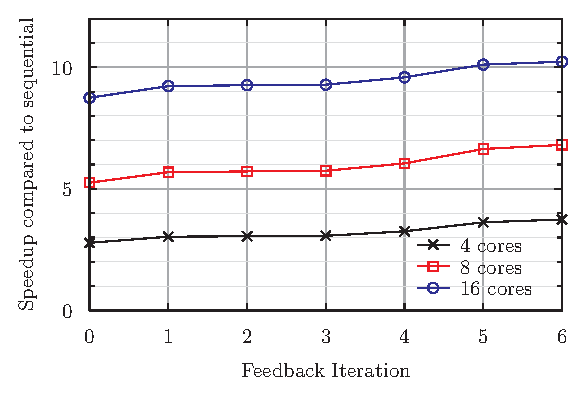
\includegraphics[width=\textwidth]{Informed/Figures/IterSum.eps}
    \caption[SE]{\texttt{SumEuler} speedup}
    \label{fig:iterSum}
\end{figure}
\vfill
\begin{figure}[H]
    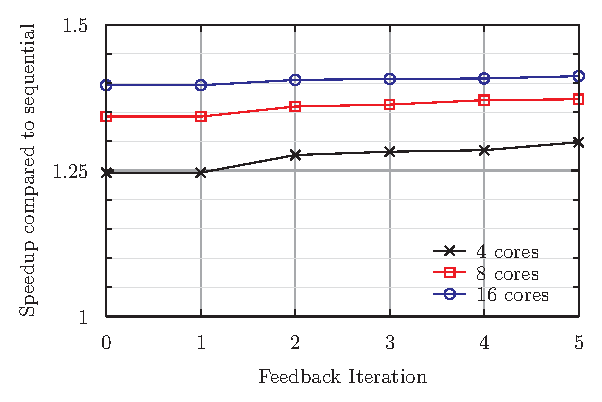
\includegraphics[width=\textwidth]{Informed/Figures/IterQueens.eps}
    \caption[Q]{\texttt{Queens} speedup}
    \label{fig:iterQueens}
\end{figure}

\clearpage

\begin{figure}[H]
    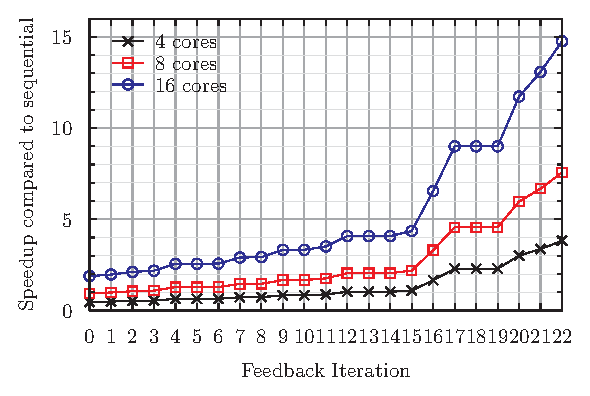
\includegraphics[width=\textwidth]{Informed/Figures/IterQueens2.eps}
    \caption[Q2]{\texttt{Queens2} speedup}
    \label{fig:iterQueens2}
\end{figure}
\vfill
\begin{figure}[H]
    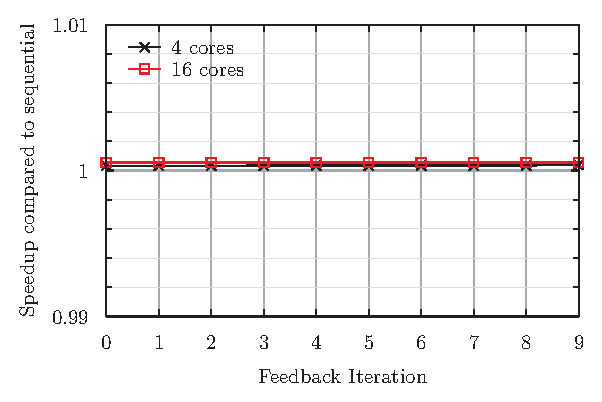
\includegraphics[width=\textwidth]{Informed/Figures/IterTaut.eps}
    \caption[T]{\texttt{Taut} speedup}
    \label{fig:iterTaut}
\end{figure}

\clearpage

Even in the cases where the final speedup is lower than anticipated, such as
\texttt{Queens} in Figure \ref{fig:iterQueens}, the program still benefits from the
iterative improvement. \texttt{Queens2} sees the highest payoff from iterative
improvement. Many of the \verb-par-s introduced by the static analysis
do not contribute significantly to the computation even though it is
semantically safe to introduce them. The iterative loop converges on the few
\verb-par- sites that make a significant difference.
